\begin{appendices}
\makeatletter
\renewcommand{\thesection}{\@arabic\c@section}  % label with numbers instead of letters
\makeatother

\section{Questionnaire}

A static print of the online questionnaire used in the study is found below.
Minor aesthetic differences are present due to conversion from a web-page,
but all content is identical.

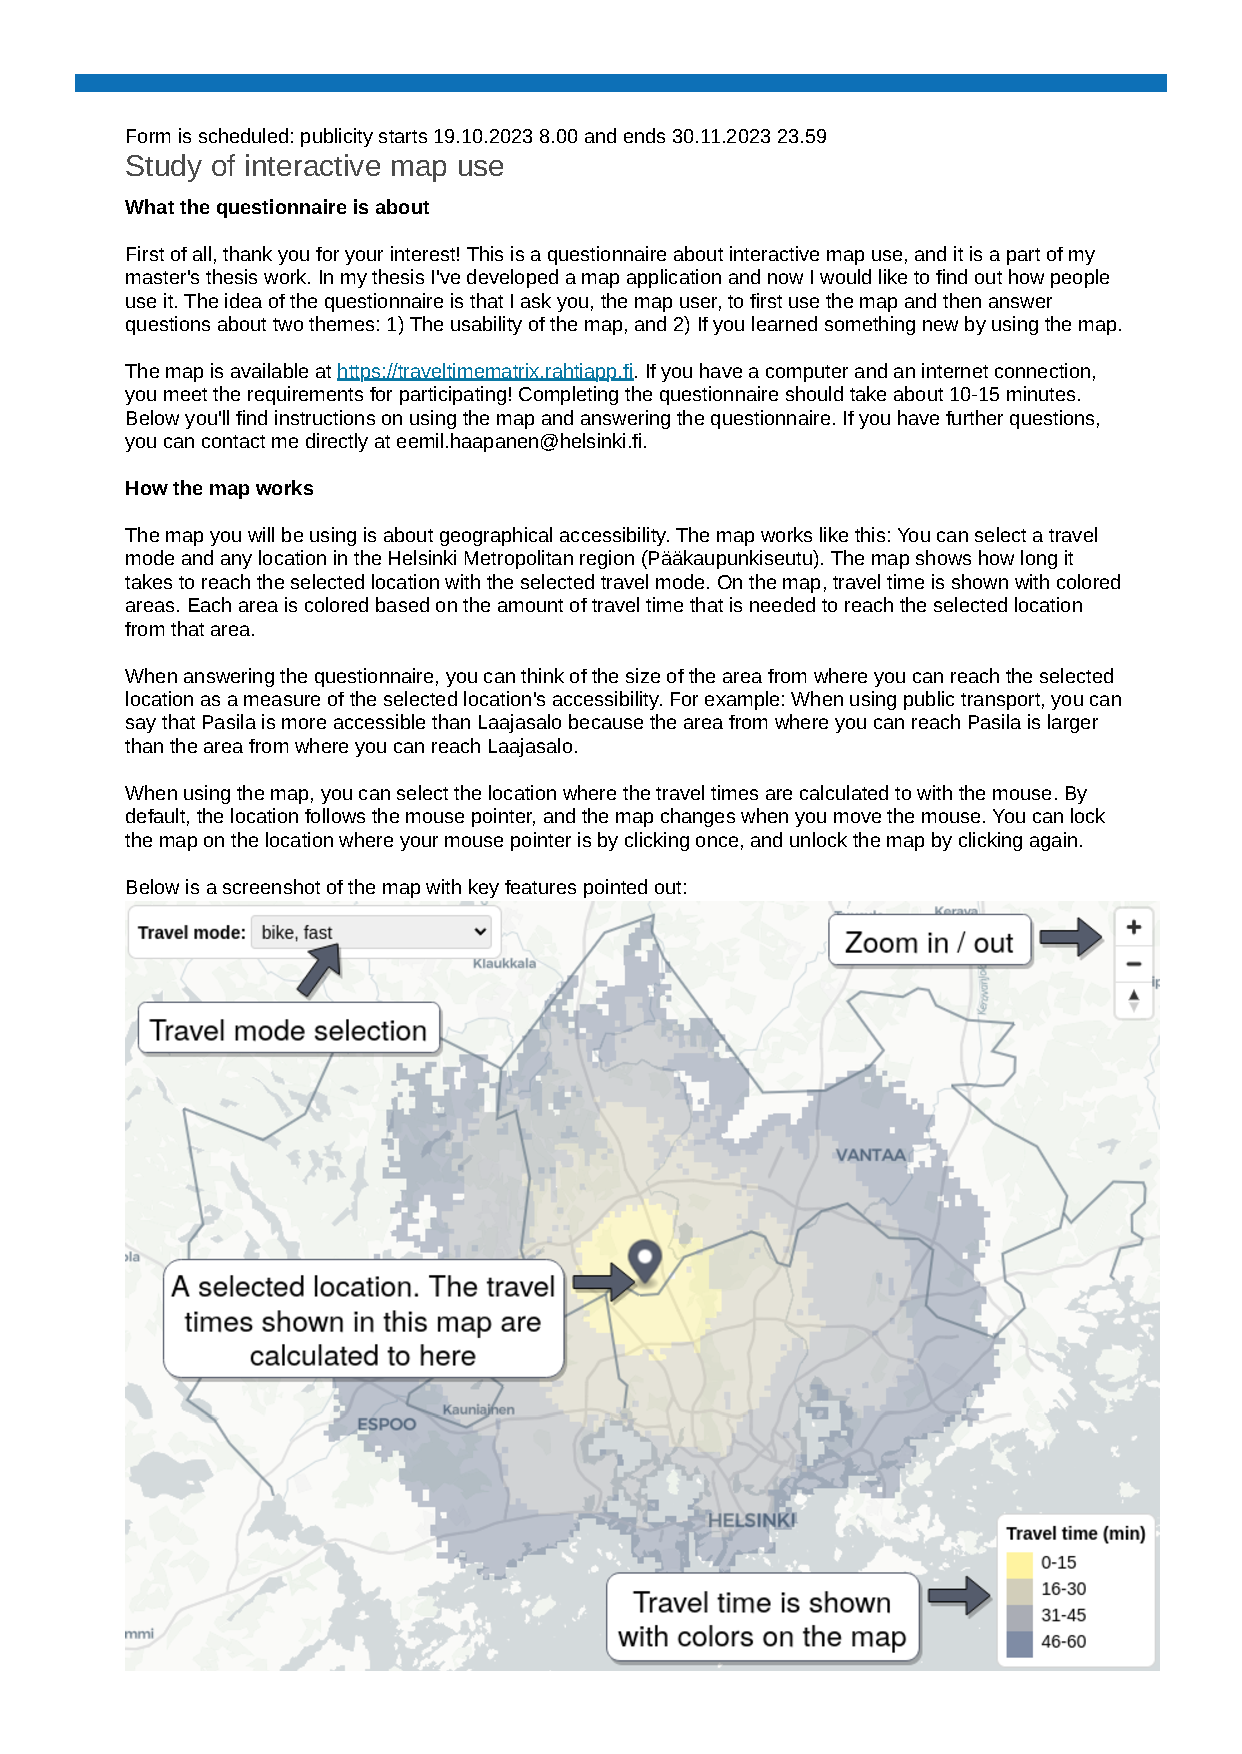
\includepdf[pages={1-},scale=1]{external_pdf/questionnaire.pdf}

\section{Questionnaire responses}

Responses to the questionnaire are presented here.
They are divided into the same task groupings that were used in the questionnaire.

\begin{figure}[H]
	% \centering
	\begin{subfigure}[b]{0.5\textwidth}
	% 	\centering
		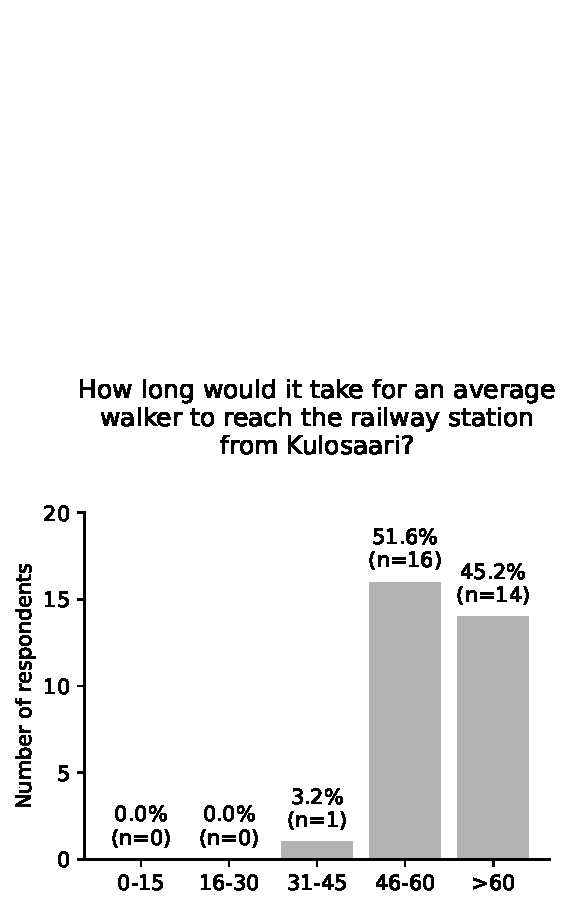
\includegraphics[width=\textwidth]{visual/figures/survey/0.pdf}
	\end{subfigure}%
	\hfill
	\begin{subfigure}[b]{0.5\textwidth}
	% 	\centering
		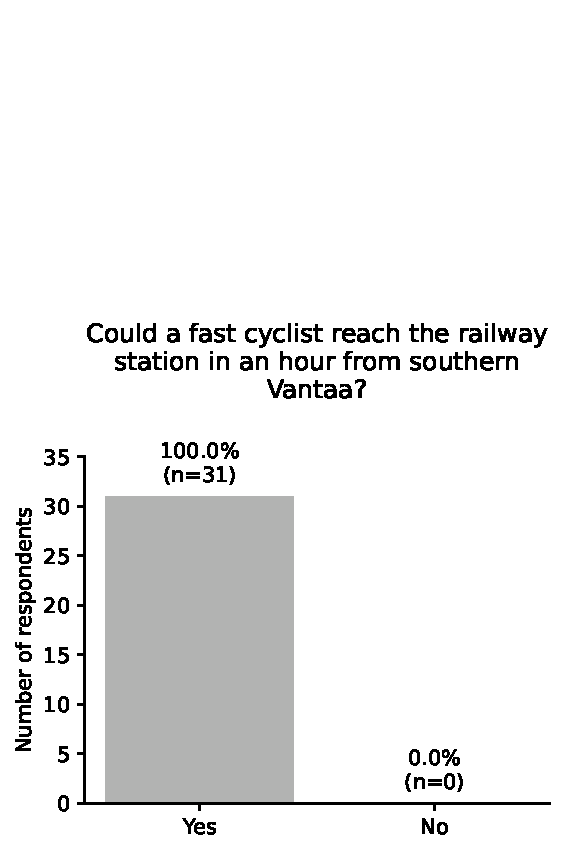
\includegraphics[width=\textwidth]{visual/figures/survey/1.pdf}
	\end{subfigure}%
	% \caption{Responses to task 1}
	% \label{fig:task 1}
	\newline
	Responses to task 1
\end{figure}

\begin{figure}[H]
	% \centering
	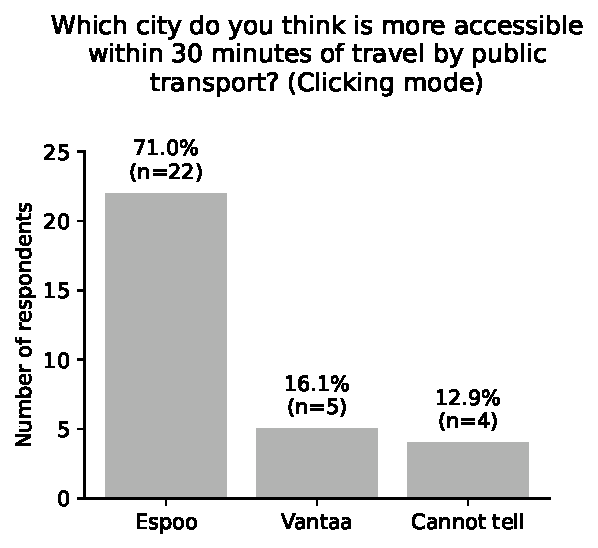
\includegraphics[width=0.5\textwidth]{visual/figures/survey/2.pdf}
	% \caption{Responses to task 2}
	% \label{fig:task 2}
	\newline
	Responses to task 2
\end{figure}

\begin{figure}[H]
	% \centering
	\begin{subfigure}[b]{0.5\textwidth}
	% 	\centering
		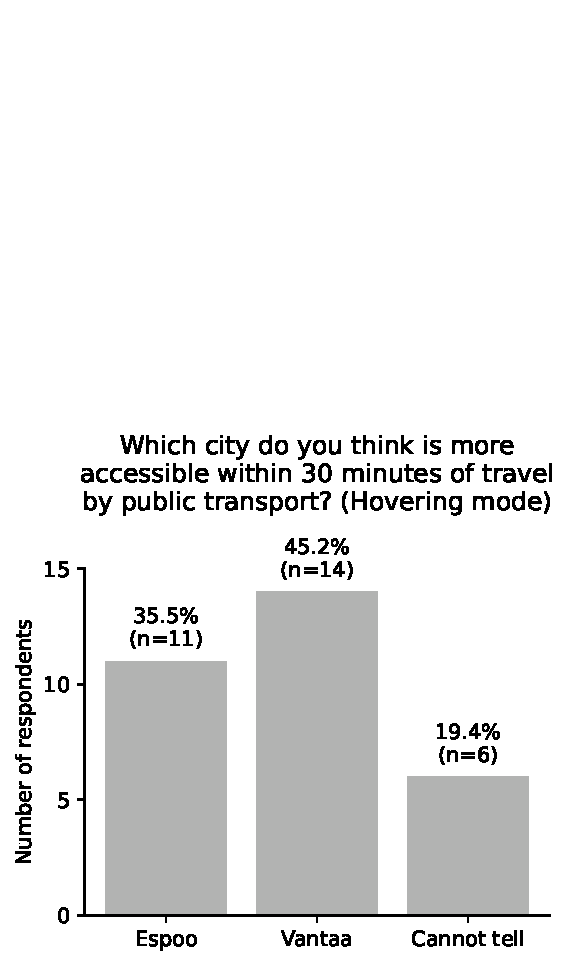
\includegraphics[width=\textwidth]{visual/figures/survey/3.pdf}
	\end{subfigure}%
	\hfill
	\begin{subfigure}[b]{0.5\textwidth}
	% 	\centering
		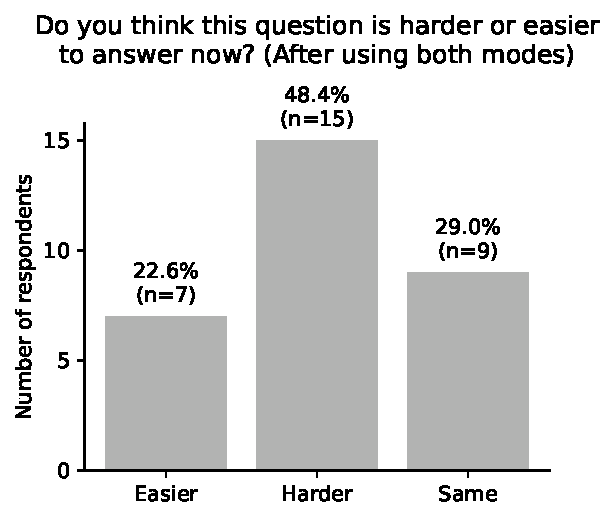
\includegraphics[width=\textwidth]{visual/figures/survey/4.pdf}
	\end{subfigure}%
	% \caption{Responses to task 3}
	% \label{fig:task 3}
	\newline
	Responses to task 3
\end{figure}

\begin{figure}[H]
	% \centering
	\begin{subfigure}[b]{0.5\textwidth}
	% 	\centering
		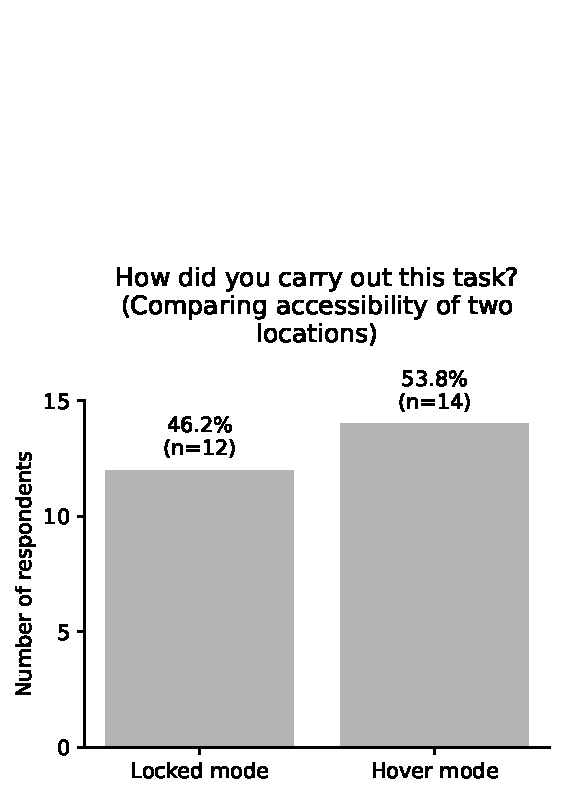
\includegraphics[width=\textwidth]{visual/figures/survey/5.pdf}
	% 	\caption{Responses to task 4}
	% 	\label{fig:task 4}
	\end{subfigure}%
	\begin{subfigure}[b]{0.5\textwidth}
	% 	\centering
		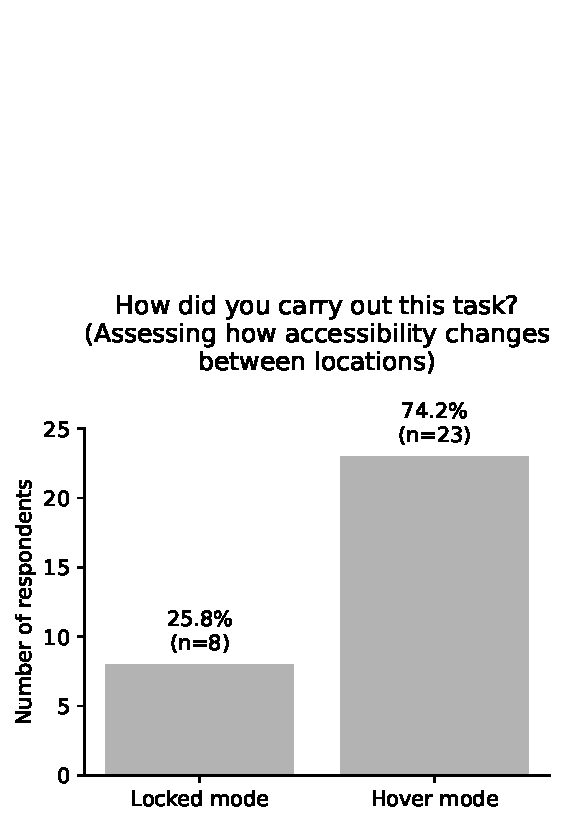
\includegraphics[width=\textwidth]{visual/figures/survey/6.pdf}
	% 	\caption{Responses to task 5}
	% 	\label{fig:task 5}
	\end{subfigure}
	\newline
	Responses to task 4
\end{figure}

\begin{figure}[H]
	% \centering
	\begin{subfigure}[b]{0.5\textwidth}
	% 	\centering
		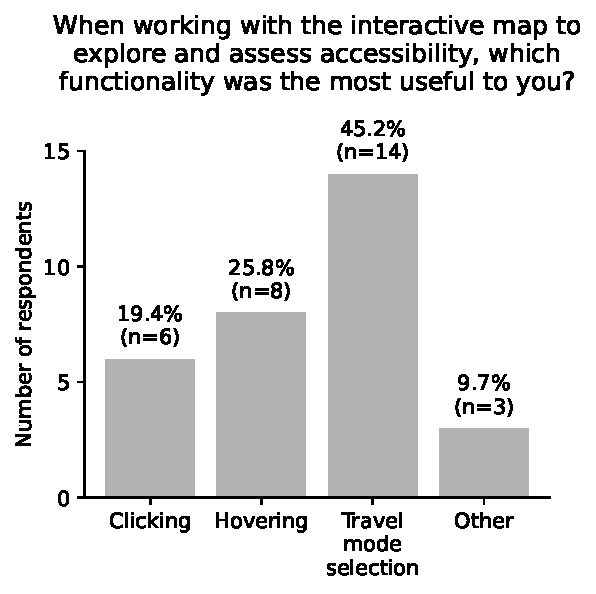
\includegraphics[width=\textwidth]{visual/figures/survey/7.pdf}
	\end{subfigure}%
	\hfill
	\begin{subfigure}[b]{0.5\textwidth}
	% 	\centering
		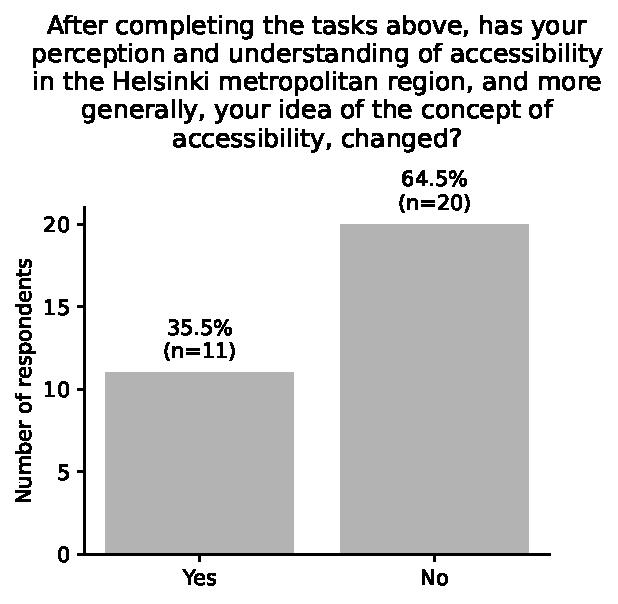
\includegraphics[width=\textwidth]{visual/figures/survey/8.pdf}
	\end{subfigure}%
	\newline
	\begin{subfigure}[b]{0.5\textwidth}
	% 	\centering
		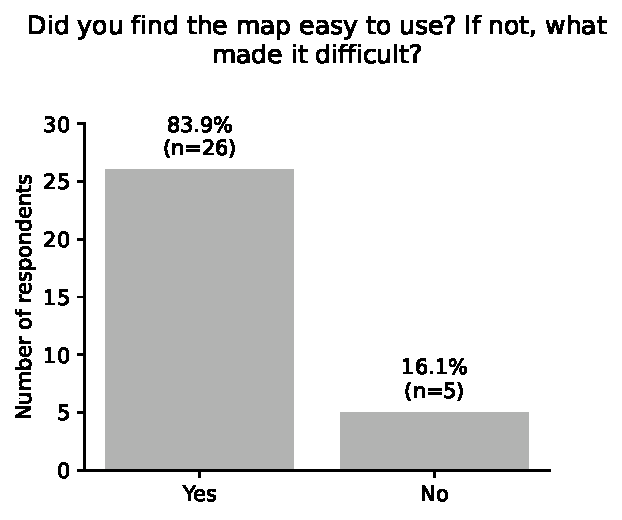
\includegraphics[width=\textwidth]{visual/figures/survey/9.pdf}
	\end{subfigure}%
	% \caption{Responses to general questions}
	% \label{fig:general questions}
	\newline
	Responses to task 5
\end{figure}

\begin{figure}[H]
	% \centering
	\begin{subfigure}[b]{0.5\textwidth}
	% 	\centering
		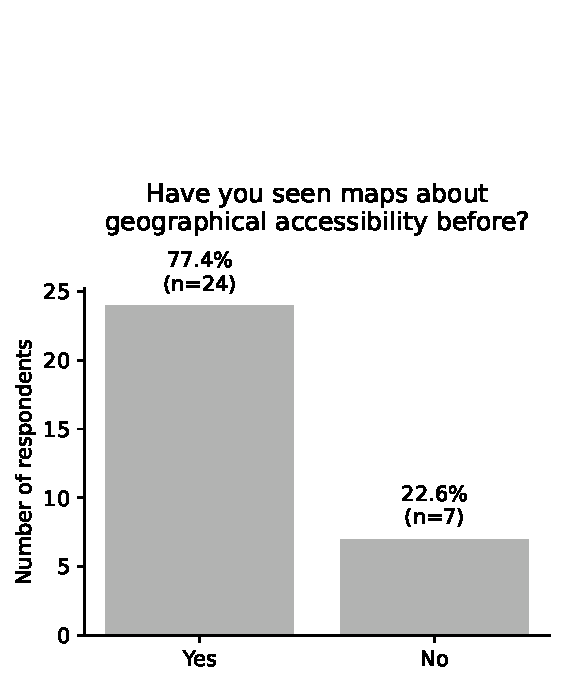
\includegraphics[width=\textwidth]{visual/figures/survey/10.pdf}
	\end{subfigure}%
	\hfill
	\begin{subfigure}[b]{0.5\textwidth}
	% 	\centering
		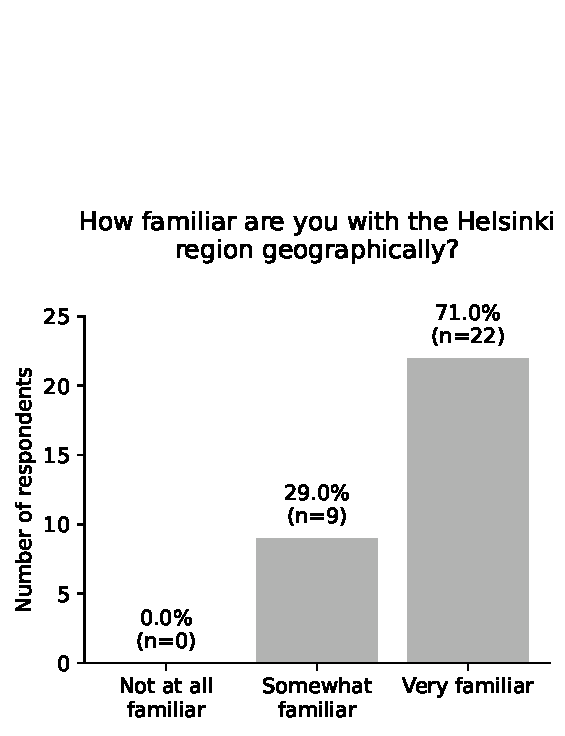
\includegraphics[width=\textwidth]{visual/figures/survey/11.pdf}
	\end{subfigure}%
	\newline
	\begin{subfigure}[b]{0.5\textwidth}  % [t] to position to top
	% 	\centering
		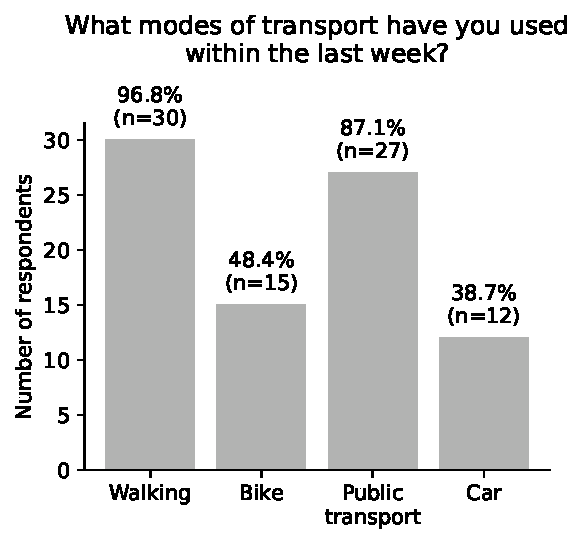
\includegraphics[width=\textwidth]{visual/figures/survey/modes.pdf}
	\end{subfigure}%
	\begin{subfigure}[b]{0.5\textwidth}
	% 	\centering
		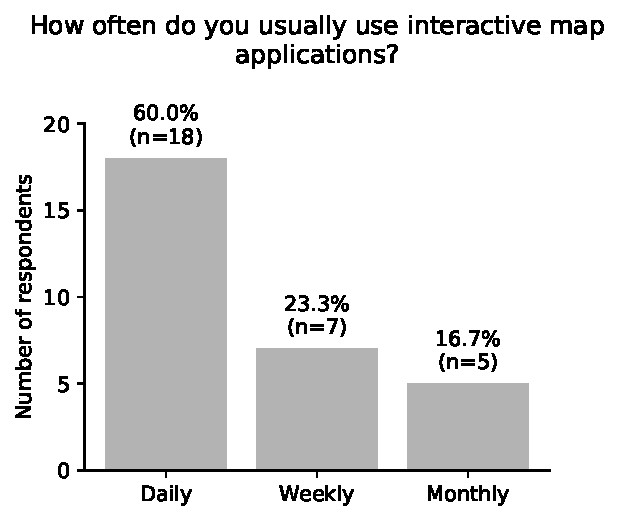
\includegraphics[width=\textwidth]{visual/figures/survey/12.pdf}
	\end{subfigure}%
	% \caption{Responses to questions about background information}
	% \label{fig:background information}
	\newline
	Responses to general questions
\end{figure}

\begin{figure}[H]
	% \centering
	\begin{subfigure}[b]{0.5\textwidth}
	% 	\centering
		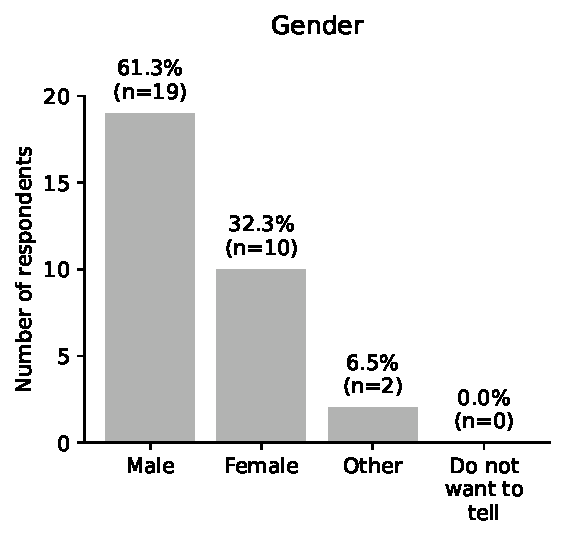
\includegraphics[width=\textwidth]{visual/figures/survey/13.pdf}
	\end{subfigure}%
	\hfill
	\begin{subfigure}[b]{0.5\textwidth}
	% 	\centering
		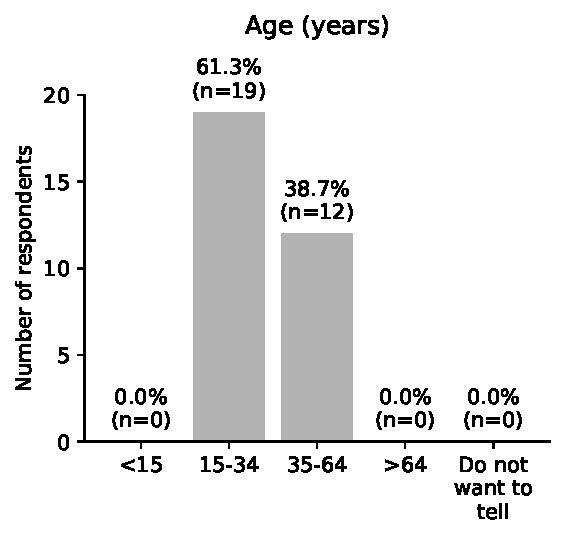
\includegraphics[width=\textwidth]{visual/figures/survey/14.pdf}
	\end{subfigure}%
	% \caption{Responses to questions about demographic information}
	% \label{fig:demographic questions}
	\newline
	Responses to questions about background information
\end{figure}

\end{appendices}
